\part{Exercises}\label{assignments}

\chapter{Exercise 0 - Identify Technologies}\label{assignment-0}

Exercise 0 will require you to identify the different software
tools/technologies included in the given attachment and then group them
into the correct layer of categories as indicated on the left-hand side
of the slide.

This homework is worth 5 points.

\slides{Assignments}{Exercise 0}{5 points}{https://drive.google.com/open?id=0B88HKpainTSfQ2FrUzdKRkM5X0U}

\chapter{Exercise 1 - Basic Statistics with Hadoop}\label{exercise-1}

%\setboolean{@twoside}{false}

\FILENAME

\section*{Basic Statistics with Hadoop}       

The idea of this exercise is to get you started with Hadoop and the
MapReduce concept. You may have already looked at the WordCount
example, both serial and Hadoop implementations. This problem is
similar to WordCount except that you will be computing the basic
statistics such as min, max, average, and standard deviation of a
given data set.

The input to the program will be a text file carrying exactly one
floating point number per line. The output should include \textit{min,
  max, average, and standard deviation} f these numbers.

\begin{figure}[!htbp]
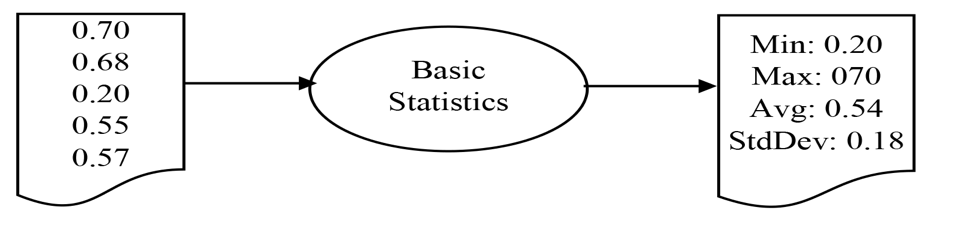
\includegraphics[width=8cm,height=3cm]{section/icloud/assignment/exercise1/p1example.png}
\centering
\end{figure}

\subsection*{Files}

A test input file is available as a separate attachment.  The
statistics values for this input are \textit{Min: 0.01 Max: 0.99 Avg:
  0.50 StdDev: 0.2817}

\slides{Assignments}{Exercise 1}{Input Data}{https://drive.google.com/open?id=0B88HKpainTSfcUlZX3BpV05TRDg}

\subsection*{Deliverables}

You will need to complete the source code and write a report. Zip your
work into a file with the name \verb|username_exercise1.zip| (replace
\textit{username} with your own) and submit the following:

\begin{itemize}
\item Complete source code
\item A document with the following details:

  \begin{itemize}
  \item	Transformation of data during the computations, i.e. data type of key, value
  \item	The data structure used to transfer between Map and Reduce phases
  \item	How the data flow happens through disk and memory during the computation
  \end{itemize}

\end{itemize}

\subsection*{Evaluation}

The point total for this exercise is 5.

\begin{itemize}
\item Correctness of the source code (2 points)
\item	Completeness of the report (3 points)
\end{itemize}



\chapter{Exercise 2 - Page Rank}\label{exercise-2}


\section*{Hadoop PageRank Cloud Computing}
 
This assignment provides an illustration of PageRank algorithms and Hadoop. You
will then blend these applications by implementing a parallel version of
PageRank using the programming interfaces of the Hadoop MapReduce framework. 


\subsection*{Deliverables}
You are required to turn in the following items in a zip file
(username\_HadoopPageRank.zip) in this assignment: 

\begin{itemize}
\item The source code of Hadoop PageRank you implemented.
\item Technical report (username\_HadoopPageRank\_report.docx) that contains: 
\item The description of the main steps and data flow in your program. 
\item The output file (username\_HadoopPageRank\_output.txt) which contains the
  first 10 urls along with their ranks. 

\end{itemize}

\subsection*{Evaluation}
The point total for this exercise is 10, where the distribution is as follows:
\begin{itemize}
\item Completeness of your code and output (7 points)
\item Correctness of written report (3 points)
\end{itemize}

\subsection*{What is PageRank?}
The web search engine is a typical distributed system on the Internet. It is
designed to search for information on the World Wide Web. The search results
are generally presented in a list of results and are often called hits.
PageRank is a well-known web graph ranking algorithm that helps Internet users
sort hits by their importance. 

PageRank calculates a numerical value for each element of a hyperlinked set of
webpages, which reflects the probability that a random surfer will access that
page. The process of PageRank can be understood as a Markov Chain which
requires iterative calculations to converge. An iteration of PageRank
calculates the new access probability for each webpage based on values
calculated in the previous iteration. The process will repeat until the number
of current iterations is bigger than predefined maximum iterations, or the
Euclidian distance between rank values in two subsequent iterations is less
than a predefined threshold that controls the accuracy of the output results. 

\begin{figure}[!htbp]
\centering
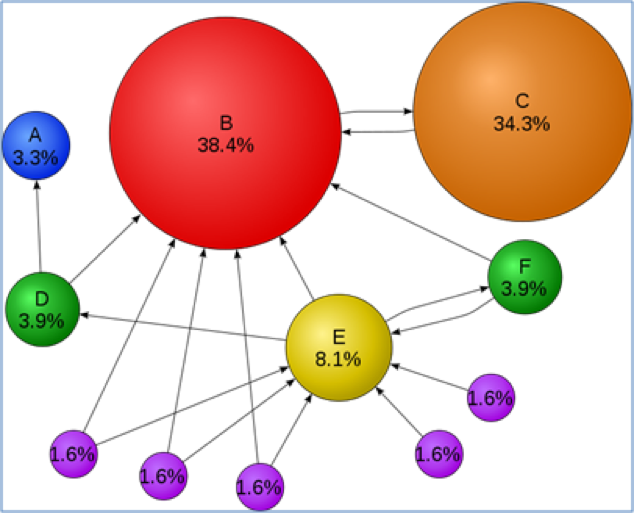
\includegraphics[width=8cm]{section/icloud/assignment/exercise2/pagerankexample}
\caption{Mathematical PageRank for a simple network in Wikipedia}
\label{fig:pagerankexample}
\end{figure}

Figure~\ref{fig:pagerankexample} shows a web graph consisting of 11 vertices
{A, B, C, D, E, F, G1, G2, G3, G4, G5}. Each vertex refers to a unique webpage,
and the directed edge means there is one link from the source webpage to the
target webpage. The percentage on each vertex represents the rank value of each
webpage.

\subsection*{Notes}

You can implement a sequential PageRank that can run on desktops or laptops.
But when processing larger input data, like web graphs containing more than a
million webpages, you need to run the PageRank application in parallel so that
it can aggregate the computing power of multiple compute nodes. Currently, in
both industry and academia, the study of large-scale web or social graphs has
become increasingly popular. In one published paper, the job execution engines
that claim to support large-scale PageRank include: MPI, Hadoop, Dryad,
Twister, Pregel. 

\subsection*{Formula}

Equation~\ref{eq:pagerank} is the formula to calculate the rank value for each
webpage. We will learn this formula by applying it to the case in
Figure~\ref{fig:pagerankexample}. There are 11 webpages in
Figure~\ref{fig:pagerankexample}, which include: {A, B, C, D, E, F, G1, G2, G3,
G4, G5}. Assuming the probability distribution for a web surfer accessing all
these 11 pages in current iteration is \{PR(A), PR(B), PR(C), ... PR(G5)\},
then the probability for the surfer to access Page B in the next iteration is:
\\

$PR(B) = PR(D)/2 + PR(E)/3 + PR(F)/2 + PR(C) + PR(G1)/2 + PR(G2)/2 + PR(G3)/2 $\\


In a general case, the PageRank value for any page u can be expressed as:

\begin{equation}\label{eq:pagerank}
PR(u) = \sum_{v \in Set} \frac{PR(V)}{L(v)}
\end{equation}

The vertices seen in the right of the formula contain all the webpages that
point to target webpage 'u'. The L(v) refers to the out degree of each webpage
in the vertices set. The initial rank values of each webpage, like PR'(u), can
be any double value. After several iteration calculations, the rank values
converge to the stationary distribution regardless of what their initial values
are.

\subsection*{Damping factor}
The PageRank theory holds that even an imaginary surfer who is randomly
clicking on links will eventually stop clicking. The probability, at any step,
that the person will continue is a damping factor d. Various studies have
tested different damping factors, but it is generally assumed that the damping
factor will be around 0.85. The formula considering damping factor is shown in
Equation~\ref{eq:pagerankwithdf}. N refers to the total number of unique urls. 

\begin{equation}\label{eq:pagerankwithdf}
PR(u) = \frac{1-d}{N} + d * \sum_{v \in Set} \frac{PR(V)}{L(v)}
\end{equation}

\section*{Hadoop PageRank DataFlow}
In this exercise, we have provided a sketch code which contains three MapReduce
jobs for you to implement:

\begin{itemize}
\item CreateGraph (done): add one column, 'initial pagerank value', to the
  input pagerank adjacency matrix (AM). Then pass it to the PageRank program to
    calculate the pagerank values. 
\item PageRank (your implementation): take the transformed AM matrix and
  calculate pagerank values for all pages. 
\item Cleanup Results: remove the targetUrls column and output
  \textbf{(sourceUrl, pagerank value)} as the final result. 
\end{itemize}

The detail dataflow can be seen in Figure~\ref{fig:hadoopdataflow}. Part 1 and
Part 3 are given as full solutions in this pipeline; you will implement the 2nd
part of the PageRank program.

\begin{figure}[!htbp]
\centering

\includegraphics[width=10cm]{section/icloud/assignment/exercise2/hadoopdataflow.png}
\caption{Hadoop PageRank dataflow}
\label{fig:hadoopdataflow}
\end{figure}

Normally for any Hadoop MapReduce program, input data is uploaded and stored in
the Hadoop Distributed File System (HDFS) before computation in order to
generate \textbf{(key, value)} pairs to the mapper. Initially, the PageRank
input data is stored in the format of adjacency matrix as a file(s) in the
local file system. Then it will be uploaded to the HDFS and distributed across
the compute nodes. Hadoop framework reads the application records from HDFS
with the InputFormat interface and generates \textbf{(key, value)} pair input
streams. Each Map function produces zero or more intermediate \textbf{(key,
value)} pairs by consuming one input (key, value) pair. For this PageRank
program, the map function applies the calculation $\frac{PR(v)}{L(V)}$ to each
\textbf{(key, value)} pair, where the key is the unique id or name of the
webpage and the value contains the current rank value of the webpage and its
out link information. Map tasks then generate intermediate (key, value) pairs,
whose value is the partial rank value of every webpage. Each reduce task
aggregates all the partial values of specific webpages by applying the provided
Equation~\ref{eq:pagerankwithdf}. The aggregated global rank values are written
back to HDFS, which in turn is used as input in the next set of iterations, if
any. "Hadoop - PageRank" in Figure~\ref{fig:hadoopdataflow} shows an example
for the PageRank data processing.


\section*{Code for Hadoop PageRank}

You need to complete two files in the provided pacakge inside
"indiana/cgl/hadoop/pagerank/": PageRankMap.java and PageRankReduce.java. Code
snapshots are shown below.

\lstinputlisting[language=Java]{section/icloud/assignment/exercise2/PageRankMap.java}
\lstinputlisting[language=Java]{section/icloud/assignment/exercise2/PageRankReducer.java}

\subsection*{Edit}
The sketch code is stored within the provided VirtualBox image. Use Eclipse or
linux text editor vi/vim to add your code.

\begin{lstlisting}[language=bash]
$ cd /root/MoocHomeworks/HadoopPageRank/
$ vim src/indiana/cgl/hadoop/pagerank/PageRankMap.java
$ vim src/indiana/cgl/hadoop/pagerank/PageRankReduce.java
\end{lstlisting}

% $ fix laout do not remove 

\subsection*{Compile and run your code}

Use the one-click script compileAndExecHadoopPageRank.sh provided below.
Standard error messages such as compile errors, execution errors, etc. will be
redirected on the screen. Debug them based on the returned messages.

\begin{lstlisting}[language=bash]
$ cd /root/MoocHomeworks/HadoopPageRank/
# usage: ./compileAndExecHadoopPageRank.sh [PageRank Input File][Number of Urls][Number Of Iterations]
$ ./compileAndExecHadoopPageRank.sh PageRankDataGenerator/pagerank5000g50.input.0 5000 1
\end{lstlisting}

\TODO{Hyungro: fix filenames with exercise not project}

\subsection*{View the result}
The result is generated as /root/hbaseMoocAntProject/output/project2.txt. 
\begin{lstlisting}[language=bash]
$ cd /root/MoocHomeworks/HadoopPageRank/
$ cat output/*
\end{lstlisting}


\chapter{Exercise 3 - Map Reduce}\label{exercise-3}

\section*{Hadoop Blast}
 
By this point you should have gone over the sections concerning Hadoop Setup
and a few Hadoop programs. Now you are going to blend these applications by
implementing a parallel version of BLAST (Basic Local Alignment Search Tool:

\URL{http://blast.ncbi.nlm.nih.gov/Blast.cgi} 

using the programming
interfaces of the Hadoop MapReduce framework. Note that this application is
written in "Map-Only" fashion, which means no reduce code is necessary.

\subsection*{Deliverables} 

You are required to turn in the following items in a zip file
(username\_HadoopBlast.zip)

\begin{itemize} 
\item The source code of Hadoop Blast you implemented.
\item	Technical report (username\_HadoopBlast\_report.docx) that answers the
  following questions.

\begin{itemize}
\item What is Hadoop Distributed Cache and how is it used in this program? 
\item Write the two lines that put and get values from Distributed cache. Also
  include the method and class information.

\item In previous exercises we used Hadoop's TextInputFormat to feed in the file
  splits line by line to map tasks. In this program, however, we want to feed
    in a whole file to a single map task. What is the technique used to achieve
    this? Also, briefly explain what are the key and value pairs you receive as
    input to a map task and what methods are responsible for producing these
    pairs?

\item Do you think this particular implementation will work if the input files
  are larger than the default HDFS block size? Briefly explain why. [Hint: you
    can test what will happen by concatenating the same input file multiple
    times to create a larger input file in the resources/blast\_input folder]

\item	If you wanted to extend this program such that all output files will be
  concatenated into a single file, what key and value pairs would you need to
    emit from the map task? Also, how would you use these in the reduce that
    you would need to add?

\end{itemize}
\item	The 4 output FASTA files: celllines\_1.fa to celllines\_4.fa.
\end{itemize}


\subsection*{Evaluation} 

The point total for this exercise is 3, where the distribution is as follows:
\begin{itemize} 
\item	Completeness of your code and output (1 points)
\item	Correctness of written report (2 points)
\end{itemize}

\subsection*{Introduction}   

Hadoop-Blast is an advanced Hadoop program which helps BLAST, a bioinformatics
application, to utilize the computing capability of Hadoop. This exercise shows
the details of its implementation, and provides an example of how to handle
similar approaches in other applications.

BLAST is one of the most widely used bioinformatics applications written in
C++. The version we are using is v2.2.23, which houses new features and better
performance. The database used in the following settings is a subset of a full
8.5GB (nr) database; its full name is Non-redundant protein sequence database.
Optionally, for more details on how to run the BLAST binary, please see Big
Data for Science tutorial page for Blast Installation [NOT required for the
assignment].

In this exercise, we have provided a sketch code which contains just one java
class for you to implement:

\begin{itemize}
\item RunnerMap.java: The pleasingly-parallel/map-only Map class which takes
the prepackaged Blast (v2.2.23) Binary Program and optimized database from
Hadoop's Distributed Cache, then executes BLAST binary as java external process
with the assigned FASTA file. These are passed as key-value pairs of
\textbf{(filename, filepath on HDFS)} handled by a provided customized Hadoop
MapReduce InputFormat DataFileInputFormat.java.  
\end{itemize}

The detail dataflow can be seen in Figure~\ref{fig:blastdataflow}. You will
implement the RunnerMap.java, which copies the distributed cache and assigned
FASTA file to local, then run the BLAST binary with correct parameters.

\begin{figure}[!htbp]
\centering
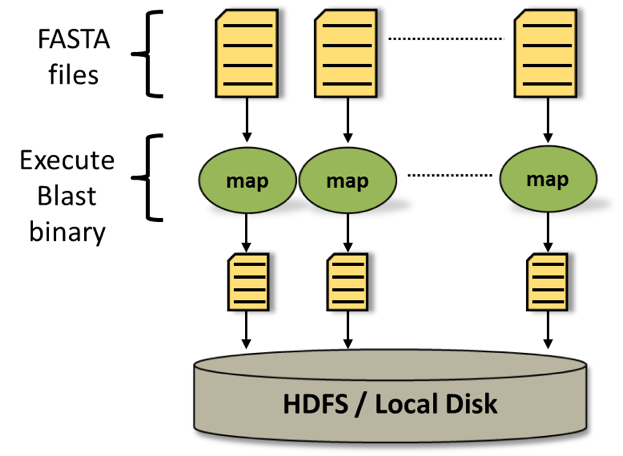
\includegraphics[width=8cm]{section/icloud/assignment/exercise3/blastdataflow}
\caption{Hadoop Blast dataflow}
\label{fig:blastdataflow}
\end{figure}

Normally, for any Hadoop MapReduce program, input data is uploaded and stored
in the Hadoop Distributed File System (HDFS) before computation in order to
generate \textbf{(key, value)} pairs to the mapper. Initially, the BLAST input
data is a set of FASTA files located in the local file system. Then it will be
uploaded to the HDFS and distributed across the compute nodes. Hadoop framework
reads the application records from HDFS with the InputFormat interface and
generates \textbf{(key, value)} pair input streams; here, we use a provided
customized Hadoop MapReduce InputFormat DataFileInputFormat.java to generate
key-value pairs of \textbf{(filename, filepath on HDFS)}. For this Hadoop Blast
program, the map function initially sets up the distributed cache and generates
the two absolute location filepaths for Blast binary and Blast Database.
Afterwards it copies the assigned FASTA file to local disk by looking up the
file from HDFS and generating an absolute filepath. Once this is accomplished
and file dependencies are stored in the local disk, we call an external java
process and execute the Blast binary with the correct parameters. Finally, the
output FASTA file of Blast binary will be uploaded back to HDFS.

\subsection*{Sketch for Hadoop Blast}
You need to complete one file in the provided pacakge inside
"cgl/hadoop/apps/runner": RunnerMap.java. Code snapshots are shown below.

\lstinputlisting[language=Java]{section/icloud/assignment/exercise3/RunnerMap.java}

In addition, if you need to understand the dataflow and main program, please
look into the DataAnalysis.java.

\lstinputlisting[language=Java]{section/icloud/assignment/exercise3/DataAnalysis.java}


\subsection*{Edit}
The sketch code is stored within the provided VirtualBox image. Use linux text
editor vi/vim to add your code.

\begin{lstlisting}[language=bash]
$ cd /root/MoocHomeworks/HadoopBlast/
$ vim src/cgl/hadoop/apps/runner/RunnerMap.java
\end{lstlisting}

\subsection*{Compile and run your code}
Use the same one-click script compileAndExecHadoopBlast.sh as in prior
homework. Standard error messages such as compile errors, execution errors,
etc. will be redirected on the screen. Follow the same debugging format.

\begin{lstlisting}[language=bash]
$ cd /root/MoocHomeworks/HadoopBlast/
$ ./compileAndExecHadoopBlast.sh 
\end{lstlisting}

\subsection*{View the result} 
The result is generated at
/root/MoocHomeworks/HadoopBlast/output/HDFS\_blast\_output . There should be 4
output FASTA files with .fa extension

\begin{lstlisting}[language=bash]
$ cd /root/MoocHomeworks/HadoopBlast/output/HDFS_blast_output
$ ls
\end{lstlisting}


\chapter{Exercise 4 - HBase Word Count}\label{exercise-4}

\section*{HBase WordCount}

\TODO{Hyungro: fix hyperlinks, use exercise instead or project where
  appropriate}
 
Write an HBase WordCount program to count all unique terms' occurrences from
the clueWeb09 dataset. Each row record of columnfamily "frequencies" is unique;
the rowkey is the unique term stored in byte format, column name is "count" and
value is the term frequency shown in all documents. Load the result to HBase
WordCountTable. Figure~\ref{fig:wordcounttablescheme} shows the schema of
WordCountTable. You will compare the results of your finished run to a correct
version we will supply to you.

\begin{figure}[!htbp]
\centering
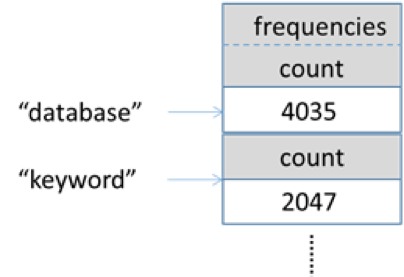
\includegraphics {section/icloud/assignment/exercise4/wordcounttablescheme}
\caption{WordCount table schema for storing unique term's occurrences}
\label{fig:wordcounttablescheme}
\end{figure}


\subsection*{Deliverables}  
Zip your source code and report in a file named username\_exercise4.zip

\subsection*{Evaluation} 

The point total for this exercise is 1.5, where the distribution is as follows:
\begin{itemize} 
\item Correctness of your code and output (1 points)
\item	Completeness of written report (0.5 points)
\item	The report should explain the logic behind your code.
\end{itemize}
 

\subsection*{Prerequisites}
You will need to load data to HBase before trying this assignment. Please follow
\textbf{instructions in HBase} for more information. 


\subsection*{Introduction}

WordCount is a simple program which counts the number of occurrences of each
word in a given text input dataset. It fits very well with the map/reduce
programming model, making WordCount a great example to understand the Hadoop
MapReduce programming style. Instead of loading the data from HDFS, we will
load our data directly from existing HBase records which store the similar
content structures on HBase and HDFS. 

In this homework and the next homework (Building an Inverted Index) we use the
same source code, which can be found in:
\textit{/root/MoocHomeworks/HBaseWordCount}.

\subsubsection*{Clueweb09 dataset}
We are using the ClueWeb09 dataset, which was created to support research on
information retrieval and related human language technologies. It consists of
about 1 billion webpages in ten languages that were collected in January and
February 2009. The dataset is used by several tracks of the TREC
conference (See~\hyperlink{link_exercise4}{Useful Links}). Since the ClueWeb09
dataset is composed of webpages crawled from the Internet, the uploaded table
schemas are designed as shown in
Figure 2.

\begin{figure}[!htbp]
\centering
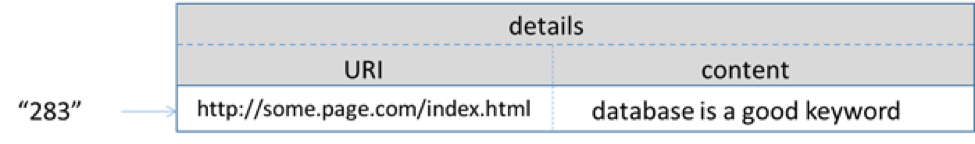
\includegraphics {section/icloud/assignment/exercise4/datatablescheme}
\caption{Data table schema for storing the ClueWeb09 dataset}
\label{fig:datatablescheme}
\end{figure}

So, while similar to Hadoop WordCount (See~\hyperlink{link_exercise4}{Useful
Links}), the differences are that data is stored on HBase and URI is the
"filename" that contains all
the text content.


\subsubsection*{Mapper, Reducer and Main Program }

Now we are going to implement the HBase WordCount. Our implementation consists
of three main parts:

\begin{itemize}
\item Mapper
\item Reducer
\item Main program
 \end{itemize}
 
 
\subsubsection*{Mapper}
A Mapper overrides the map function from the Class
"org.apache.hadoop.hbase.mapreduce.TableMapper$<$Text, LongWritable$>$" which
provides $<$key, value$>$ pairs as the input. A Mapper implementation may
output $<$key, value$>$ pairs using the provided Context.  $<$key, value$>$ of
this map function is $<$rowkey, content$>$, where the key is the rowkey of an
HBase record related to a specified URI, and the content is the stored text of
that URI. Your Map task should output $<$word, frequency$>$ for each word in
the content of text.

\textit{Pseudocode}
\begin{lstlisting}[language=java] 
void Map (key, value){
    for each word x in the content of a hbase record:
    context.write(x, freq);
}
\end{lstlisting}
 
\textit{Detailed implementation}
\begin{lstlisting}[language=java] 
static class WcMapper extends TableMapper<Text, LongWritable> {
		@Override
		public void map(ImmutableBytesWritable row, Result result, Context context) throws IOException, InterruptedException {
			byte[] contentBytes = result.getValue(Constants.CF_DETAILS_BYTES, Constants.QUAL_CONTENT_BYTES);
			String content = Bytes.toString(contentBytes);
			
			// TODO: write your implementation for counting words in each row, and generating a <word, count> pair
			// Hint: use the "getWordFreq" function to count the frequencies of words in content
 
		}
}
\end{lstlisting}

\subsubsection*{Reducer}
A Reducer collects the intermediate $<$key, value$>$ output from multiple map
tasks and assembles a single result. Here, the reducer function will sum up the
occurrence of each word to pairs as $<$word, occurrenc$e>$, then write it back
to an HBase table with put operations which contain the key-value pair
information of each word.

\textit{Pseudocode}
\begin{lstlisting}[language=java] 
void Reduce (keyword, <list of value>){
    for each x in <list of value>:
        sum+=x;
        context.write(rowkey(x), freq);
}
\end{lstlisting}

\textit{Detailed implementation}
\begin{lstlisting}[language=java] 
public static class WcReducer extends TableReducer<Text, LongWritable, ImmutableBytesWritable> {
    	@Override
    public void reduce(Text word, Iterable<LongWritable> freqs, Context context)
                throws IOException, InterruptedException {
        /*TODO: write your implementation for getting the final count of each word
        and putting it into the word count table 
        Hint -- the schema of the WordCountTable is: 
           rowkey: a word, column family: "frequencies", 
           column name: "count", cell value: count of the word
        Check iu.pti.hbaseapp.Constants for the constant values to use.
	*/
    	long totalFreq = 0;
     }
}
 \end{lstlisting}
\subsubsection*{Main program }
The main function has been provided as standard initialization, although you
can modify it to suit your own style. Hint: the provided code is designed for
using put operations in the reducer content.write() function. Before writing
the codes, please read the HBase MapReduce tutorial first
(See~\hyperlink{link_exercise4}{Useful Links}).



%\lstinputlisting[language=Java]{RunnerMap.java}

\subsection*{Edit}
 The sketch code is stored within the provided VirtualBox image Environment
 Setup. You may use linux text editor vi/vim to add your code.

\begin{lstlisting}[language=bash] 
$ cd /root/MoocHomeworks/HBaseWordCount/
$ vim src/iu/pti/hbaseapp/clueweb09/WordCountClueWeb09.java
uend{lstlisting}
 
\subsection*{Compile and run your code}
For your convenience, we have provided a one-click script
compileAndExecWordCount.sh for compiling and execution. Standard error messages
such as "compile errors, execution errors, etc." will be redirected on the
screen. You may debug it based on the returned messages.

\begin{lstlisting}[language=bash] 
$ cd /root/MoocHomeworks/HBaseWordCount
$ ./compileAndExecWordCount.sh
\end{lstlisting}
 
\subsection*{View the result}  
The result is generated as
/root/MoocHomeworks/HBaseWordCount/output/project1.txt. 

\begin{lstlisting}[language=bash] 
$ cd /root/MoocHomeworks/HBaseWordCount
$ cat output/project1.txt
\end{lstlisting}

\subsection*{Useful Links}
\begin{itemize}
  \item \href{http://hbase.apache.org/}{HBase official website}\hypertarget{link_exercise4}
  \item \href{http://lemurproject.org/clueweb09}{Clueweb09 dataset}
  \item \href{http://hbase.apache.org/book/mapreduce.example.html}{HBase MapReduce Examples}
  \item \href{http://salsahpc.indiana.edu/csci-b649-spring-2014/projects/project1.html}{Hadoop WordCount}
\end{itemize} 


% \includepdf[pages=-,pagecommand={},width=\textwidth]{section/icloud/assignment/deprecated/exercise4_pre.pdf}

\chapter{Exercise 5 - HBase Index Builder}\label{exercise-5}

\section*{HBase FreqIndexBuilder}

\TODO{Hyungro: fix exercise and replace project where appropriate.}

Write an HBase FreqIndexBuilder program to build an inverted index table which
has the unique term's occurrences in all documents from the clueWeb09 dataset.
Each row record of columnfamily ``frequencies'' is unique, where the rowkey is
the unique term stored in byte format, column name is the documentId that
contains this term, and value is the term frequency shown per document. Note
that each row has multiple columns. The result must be loaded to HBase
clueWeb09IndexTable. Figure 1 shows the schema of clueWeb09IndexTable.

\begin{figure}[!htbp]
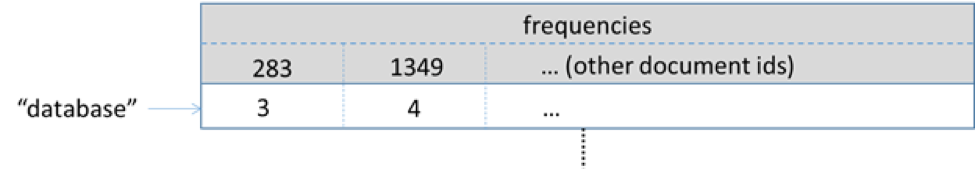
\includegraphics[width=8cm,height=1.5cm]{section/icloud/assignment/exercise5/p5-1}
\centering
\caption{clueWeb09IndexTable table schema for storing term frequencies and their related documentId}
\end{figure}

\subsection*{Deliverables}
Zip your source code, results and report in a file named
username\_exercise5.zip. Submit this file to the Canvas submission page.

\begin{itemize}
\item Complete source code
\item A written report describing the main steps
\end{itemize}

\subsection*{Evaluation}
The point total for this exercise is 3, where the distribution is as follows:
\begin{itemize}
\item Completeness of your code and output (2 points)
\item Correctness of written report (1 points)
\end{itemize}

\subsection*{Introduction}
HBase FreqIndexBuilder is an advanced WordCount program which counts the number
of occurrences of each word in a given text input dataset and also stores the
related document name (identification number) as HBase inverted index records.
These Inverted indices for text data are built for supporting efficient
searches in a huge set of text data.

\subsection*{What is Inverted Index?}
Figure 2 shows an example of an inverted index. For a given set of documents,
each composed of a series of terms (words), it records the following
information: for each term, which subset of documents contains it in their
texts.

To build these inverted indices, we reuse the ClueWeb09 dataset from before,
which was created to support research on information retrieval and related
human language technologies. The dataset is used by several tracks of the TREC
conference. New inverted index table schemas are designed as shown in Figure 1.

In the clueWeb09IndexTable table each term will have the same structure, with
term as rowkey, values contained in documentId, and the occurrence of the term
within this document shown. Our goal is to write an HBase program which
generates an inverted index table by extracting the information from the
ClueWeb09 dataset.

\begin{figure}[!htbp]
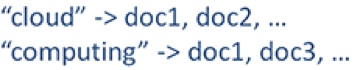
\includegraphics[width=5cm,height=1cm]{section/icloud/assignment/exercise5/p5-2}
\centering
\caption{A sample inverted index}
\end{figure}

\subsection*{Mapper and Main Program}
Now we are going to implement the HBase FreqIndexBuilder program. As opposed to
WordCount, our implementation only consists of two main parts:

\begin{itemize}
\item Mapper
\item Main program
\end{itemize}
This type of application is called ?Map-Only? parallel application.

\subsubsection*{Mapper}
A Mapper overrides the ``map'' function from the Class ``org.apache.hadoop.hbase.mapreduce.TableMapper\\
\textless Text, LongWritable\textgreater'', which provides \textless key, value\textgreater pairs as the input. A Mapper implementation may output \textless key,value\textgreater pairs using the provided Context.
\textless key, value\textgreater of this map function is \textless rowkey, content\textgreater, where the key is the rowkey of an HBase record related to a specified URI, and the content is the stored text of that URI. Your Map task should output \textless word, \textless docId, frequency\textgreater\textgreater for each word in the content of text.

\subsubsection*{Pseudocode}
\begin{lstlisting}[language=Java]
void Map(key, value) {
    for each word x in the content of a hbase record:
    context.write(x, );
}
\end{lstlisting}

\subsubsection*{Detailed implementation}
\lstinputlisting[language=Java]{section/icloud/assignment/exercise5/FibMapper.java}

\subsection*{Main Program}
Again, the main function has been provided as standard initialization, and you
may modify it to fit your own style. See the examples of using
TableMapReduceUtil.initTableMapperJob and
TableMapReduceUtil.initTableReducerJob.

\subsection*{Edit, compile and run your code}
The sketch code is stored within the provided VirtualBox image. You can use
linux text editor vi/vim to add your code.

\begin{lstlisting}[language=bash]
$ cd /root/MoocHomeworks/HBaseInvertedIndexing/
$ vim src/iu/pti/hbaseapp/clueweb09/FreqIndexBuilderClueWeb09.java
$ cd /root/MoocHomeworks/HBaseInvertedIndexing/
$ ./compileAndExecFreqIndexBuilderClueWeb.sh
\end{lstlisting}

\section*{View the result}
The result is generated as /root/hbaseMoocAntProject/output/project2.txt. 
\begin{lstlisting}[language=bash]
$ cd /root/MoocHomeworks/HBaseInvertedIndexing/
$ cat output/project2.txt
\end{lstlisting}



\chapter{Exercise 6 - Search Engine  }\label{exercise-6}

\section*{Test Search Engine}

After having familiarized yourself with the ``HBase Building an Inverted
Index'' homework and ``PageRank algorithms'' homework, you are ready to use
these applications to test the search engine function from the packaged
executable.

\subsection*{Deliverables}
Zip your source code, library, and results in a file named
username@test-search-engine.zip. Please submit this file to the Canvas
Assignments page.

\subsection*{Evaluation}
The point total for this exercise is 6, where the distribution is as follows:
\begin{itemize}
\item Completeness of your code (5 points)
\item Correct output (1 points)
\end{itemize}

\subsection*{Search Engine Implementation}
Before we test the search engine, we need to write the PageRank output to the
HBase clueWeb09PageRankTable.

\begin{lstlisting}[language=bash]
$ export HADOOP_CLASSPATH=`/root/software/hbase-0.94.7/bin/hbase classpath'
$ hadoop jar /root/software/hadoop-1.1.2/lib/cglHBaseMooc.jar  iu.pti.hbaseapp.clueweb09.PageRankTableLoader  /root/MoocHomeworks/HBaseInvertedIndexing/resources/en0000-01and02.docToNodeIdx.txt  /root/MoocHomeworks/HBaseInvertedIndexing/resources/en0000-01and02_reset_idx_and_square_pagerank.out
\end{lstlisting}

Now, combined with ``Building an Inverted Index'', we have built three database
tables on HBase:

\begin{itemize}
\item clueWeb09DataTable
\item clueWeb09IndexTable
\item clueWeb09PageRankTable
\end{itemize}

The data-flow of the program is shown in Figure 1.

\begin{figure}[!htbp]
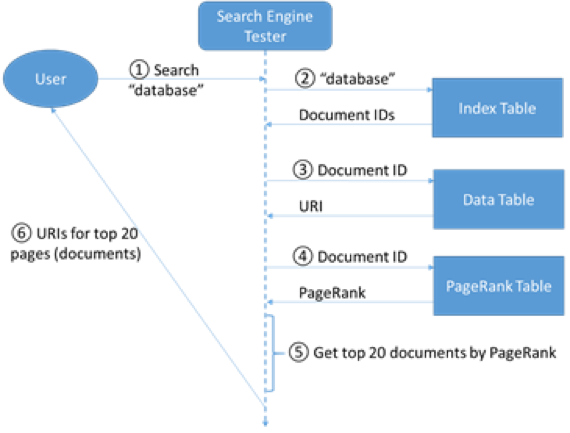
\includegraphics[width=8cm,height=6cm]{section/icloud/assignment/exercise6/p6}
\centering
\caption{Dataflow for searching keyword ``database'' among the constructed databases}
\end{figure}

You need to complete the following code before you can run the search engine:
\begin{lstlisting}[language=bash]
$ vim src/iu/pti/hbaseapp/clueweb09/SearchEngineTester.java
\end{lstlisting}

\lstinputlisting[language=Java]{section/icloud/assignment/exercise6/SearchEngineTester.java}

\section*{Compile and Run the Program}
\begin{lstlisting}[language=bash]
$ cd /root/MoocHomeworks/HBaseInvertedIndexing/
$ vim src/iu/pti/hbaseapp/clueweb09/SearchEngineTester.java
$ cd /root/MoocHomeworks/HBaseInvertedIndexing/
$ ant
$ cp /root/MoocHomeworks/HBaseInvertedIndexing/dist/lib/cglHBaseMooc.jar /root/software/hadoop-1.1.2/lib/
\end{lstlisting}

Now you can test the functionality of the search engine by running the program
with keywords.

\begin{lstlisting}[language=bash]
$ cd /root/software/hadoop-1.1.2/
$ ./bin/hadoop jar lib/cglHBaseMooc.jar  iu.pti.hbaseapp.clueweb09.SearchEngineTester search-keyword snapshot
$ ./bin/hadoop jar lib/cglHBaseMooc.jar  iu.pti.hbaseapp.clueweb09.SearchEngineTester get-page-snapshot 00000113548 |  grep snapshot
\end{lstlisting}

\subsection*{What is next?}
Congratulations, you have finished the search engine exercise!


\chapter{Exercise 7 - Harp Page Rank Map Reduce}\label{exercise-7}

\section*{Harp PageRank}

For this exercise you will implement PageRank on Harp framework.

\subsection*{Deliverables}
Zip your source code and output as username\_harp-pagerank.zip. Please submit
this file to the Canvas Assignments page.

\subsection*{Evaluation}
The point total for this exercise is 6, where the distribution is as follows:


\begin{itemize}
\item Completeness of your code (5 points)
\item Correct output (1 point)
\end{itemize}

\subsection*{Prerequisites}
From now on, you don't need the old VM. To avoid any conflict and
inconvenience, we have prepared a new VM (ubuntu 16.04) for you. The link will
be posted on canvas. All necessary tools/libaries such Maven, JDK, Github,
Hadoop 2.6.0, Harp are configured and ready for use. Intellij is installed as
well. You can also use your own VM. But you will need to setup those
tools/libraries by yourself. Some tutorials are available at the harp
website. Here this instruction is based on the configurations in
this new VM.

\begin{figure}[!htbp]
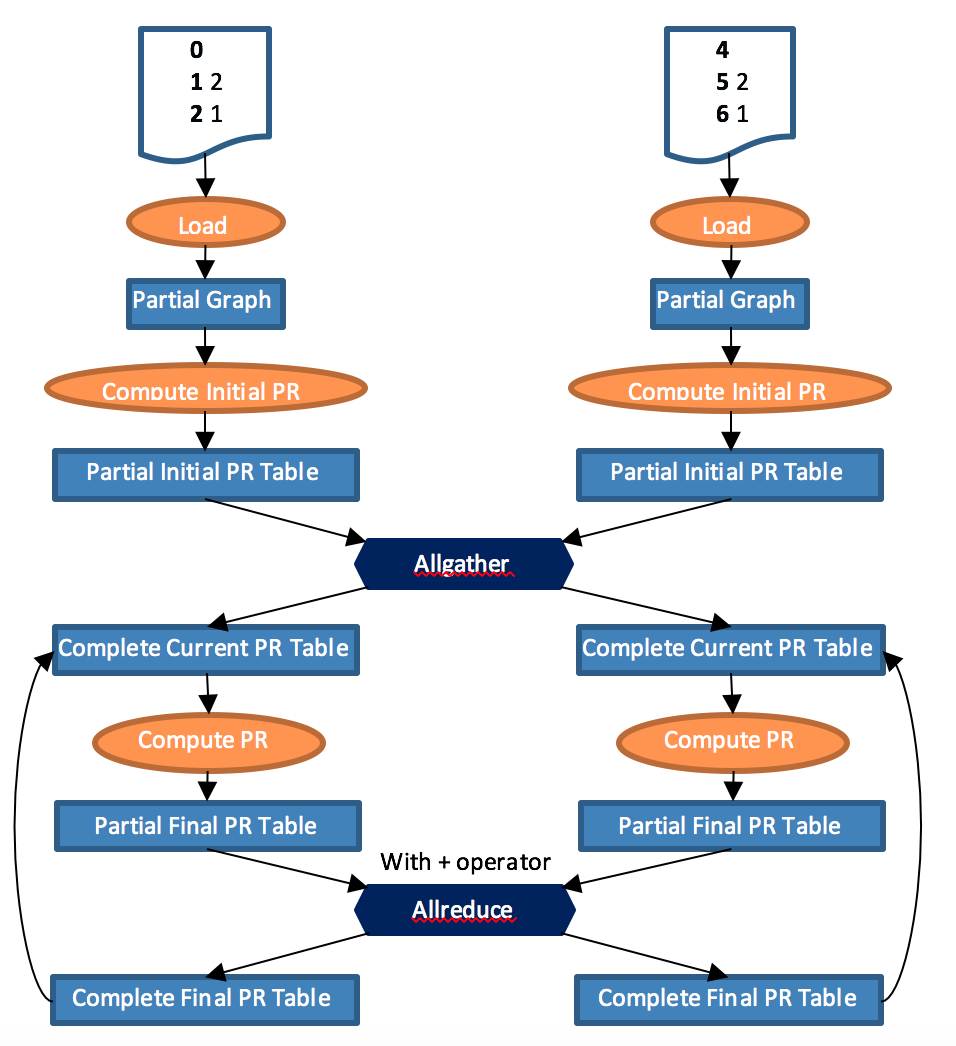
\includegraphics[width=6cm,height=8cm]{section/icloud/assignment/exercise7/p8}
\centering
\caption{Harp PageRank Architecture}
\end{figure}

\subsection*{HarpPageRank Implementation}
Most of the code is completed for you and your task will be to perform the
\textbf{Compute PR} step in the above diagram. The code for this can be found
in \textbf{simplepagerank/PageRankMapper.java}

\lstinputlisting[language=Java]{section/icloud/assignment/exercise7/computePartialPR.java}

\subsection*{Compilation and Running}
\begin{itemize}
\item To make the modification to the code, you can use Intellij IDE or linux
  terminal. The source code is located at 
\begin{lstlisting}[language=bash]
/home/cc/Documents/harp/harp-tutorial-app/src/main/java/edu/iu/simplepagerank
\end{lstlisting}
\item To compile the code, type the following commands in terminal
\begin{lstlisting}[language=bash]
$ cd $HARP_ROOT_DIR
$ mvn clean package
\end{lstlisting}

\item If hadoop is not started, start hadoop by:
\begin{lstlisting}[language=bash]
$ $HADOOP_HOME/sbin/start-dfs.sh
$ $HADOOP_HOME/sbin/start-yarn.sh
\end{lstlisting}

Then you can view the web UI at  localhost:50070 and localhost:8088

\item We prepared the input dataset (input5K-2partitions) for you. Use the
  following command to put it to hdfs. Please note there is a "dot" at the end
    of the second command.

\begin{lstlisting}[language=bash]
$ cd $HARP_ROOT_DIR/data/tutorial/simplepagerank
$ hdfs dfs -put input5K-2partitions .
\end{lstlisting}
\item Run the program:
\begin{lstlisting}[language=bash]
$ cd $HARP_ROOT_DIR
$ hadoop jar harp-tutorial-app/target/harp-tutorial-app-1.0-SNAPSHOT.jar edu.iu.simplepagerank.HarpPageRank input5K-2partitions output5k 5000 10
\end{lstlisting}

This will run PageRank against input2K-2partitions dataset. It has 5000 URLs in total. The program will run 2 parallel map tasks for 10 iterations.  If you want to launch N map tasks, you need to divide the dataset into N partitions.

\item To get the output, perform the following commands to get the output to the Desktop. Then you can submit it to canvas.
\begin{lstlisting}[language=bash]
$ hdfs dfs -get output5k /home/cc/Desktop
\end{lstlisting}
\end{itemize}


\chapter{Exercise 8 - Harp Kmeans}\label{exercise-8}

\section*{Harp Mini\-Batch Kmeans}

\TODO{Hyungro: check hyperlinks}

The goal for this exercise is to implement Harp Mini-batch Kmeans
from scratch (See~\hyperlink{link_exercise8}{Useful Links}). 

\subsection*{Deliverables}
Zip your source code and report as username\_mbkmeans.zip. Please submit this
file to the Canvas Assignments page.

\subsection*{Evaluation}

The point total for this exercise is 6, where the distribution is as
follows:

\begin{itemize}
\item Completeness of your code (5 points)
\item In the report, describe your implementation and the output. (1 points)
\end{itemize}

You can get up to 4 bonus points based on your extra efforts.

\section*{Bonus credits}

Some options you may consider to get extra credits: 

\begin{itemize}
\item Perform experiments on various (small, medium, large, etc)
  datasets
\item Test your algorithm on at least 2 nodes on FutureSystem.
\item Implement mini-batch kmeans using other tools/platforms (Spark,
  Flink, etc) and compare the performance between different
  tools/platforms (See~\hyperlink{link_exercise8}{Useful Links}).
\end{itemize}

You are encouraged to explore other options to get extra
credits. Remember to present all of your extra work in the report.
 
\subsection*{Dataset}

You can implement a script to generate data randomly as your input
datasets.  You are also free to use public datasets such as RCV1-v2
(See~\hyperlink{link_exercise8}{Useful Links}).
  
\subsection*{Mini-batch Kmeans}

You can refer to the paper for sequential mini-batch kmeans
algorithm. You will need to design how to parallelize the algorithm so
that it can run with large scale datasets on distributed computing
environment.

\begin{figure}[htb]
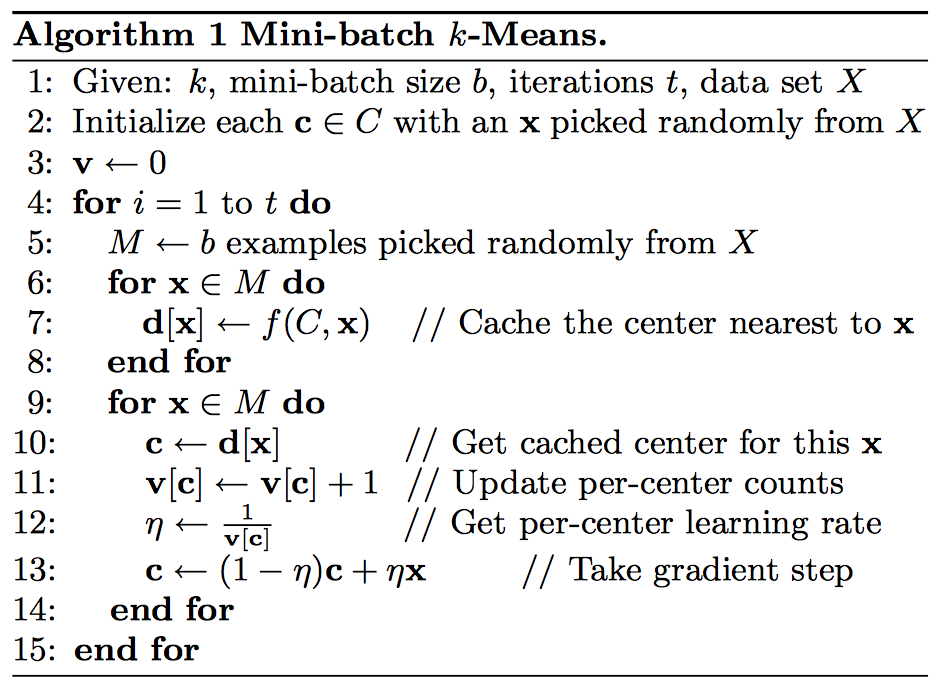
\includegraphics[width=8cm]{section/icloud/assignment/exercise8/mbkmeans}
\centering
\caption{Mini-batch Kmeans.}
\end{figure}  

\subsection*{Useful Links}

\begin{itemize}
  \item \href{http://jmlr.csail.mit.edu/papers/volume5/lewis04a/lewis04a.pdf}{RCV1: A New Benchmark Collection for Text Categorization Research} \hypertarget{link_exercise8}
  \item \href{https://dsc-spidal.github.io/harp}{Harp}
  \item \href{http://spark.apache.org}{Spark}
  \item \href{https://flink.apache.org}{Flink}
  \item \href{https://dl.acm.org/citation.cfm?id=1772862}{Web-scale k-means clustering - D. Sculley}
\end{itemize}

